\section{Mass, CG, Inertia and Static Margin}

The structural layout is defined nose to tail in \texttt{DadosCGInerciaComum.m}. The convention is $x=0$ at the nose tip, positive forward, so all section positions are negative.

\begin{table}[H]
\centering
\caption{Structural layout (nose to tail).}
\begin{tabular}{lccp{0.34\textwidth}}
\toprule
Section & Length & Mass & Role \\
\midrule
Cont (guidance/nose) & $1.09~\text{m}$ & $201~\text{kg}$ & seeker + ballast to move CG forward \\
CDG (warhead) & $0.90~\text{m}$ & $165~\text{kg}$ & payload \\
Sustainer & $2.35~\text{m}$ & $60+330$ prop & cruise motor \\
Booster & $1.25~\text{m}$ & $35+125$ prop & acceleration motor \\
Nozzle & $0.20~\text{m}$ & $14~\text{kg}$ & --- \\
\bottomrule
\end{tabular}
\end{table}

The launch mass is $M_0\approx 930~\text{kg}$ (empty $475~\text{kg}$ + propellant $455~\text{kg}$). The CG migrates forward as propellant burns and is recomputed in five burn phases: $x_{cg,0}=-2.65~\text{m}\rightarrow-1.70~\text{m}$ at burnout. Inertia is recomputed per phase ($I_{xx}$ from a solid cylinder, $I_{yy}=I_{zz}$ by parallel axis over the sections).

\subsection{Static Margin and Maximum Maneuver (Gmax)}

The static margin is the distance in calibers between CG and neutral point:
\[
    \text{margin}=\frac{x_{CG}-x_{CP}}{D_{ref}}.
\]
More margin means more stability but less maneuverability. With $x_{cg,0}=-2.65~\text{m}$ the margin is $\approx 1.1$ cal. A more rearward CG ($-2.75~\text{m}$, $\approx 0.79$ cal) forces trim to $\alpha\approx-21^\circ$, outside $\pm 20^\circ$, so the fin cannot trim it; moving the CG forward to $-2.65~\text{m}$ drops trim to $\approx-18^\circ$ and every burn phase closes within $\pm 20^\circ$.

For each CG phase and Mach, the maximum maneuver is found by solving $C_m=0$ at maximum fin ($20^\circ$) for the trim $\alpha$, then converting to $g$:
\[
    G_{max}=\frac{\bar q\,S\,C_N(\alpha_{trim})}{m\,g}.
\]
The result ranges $2\rightarrow 7.4g$ across CG phases; the terminal value is $\approx 5.6g\geq 5g$.

\begin{figure}[H]
\centering
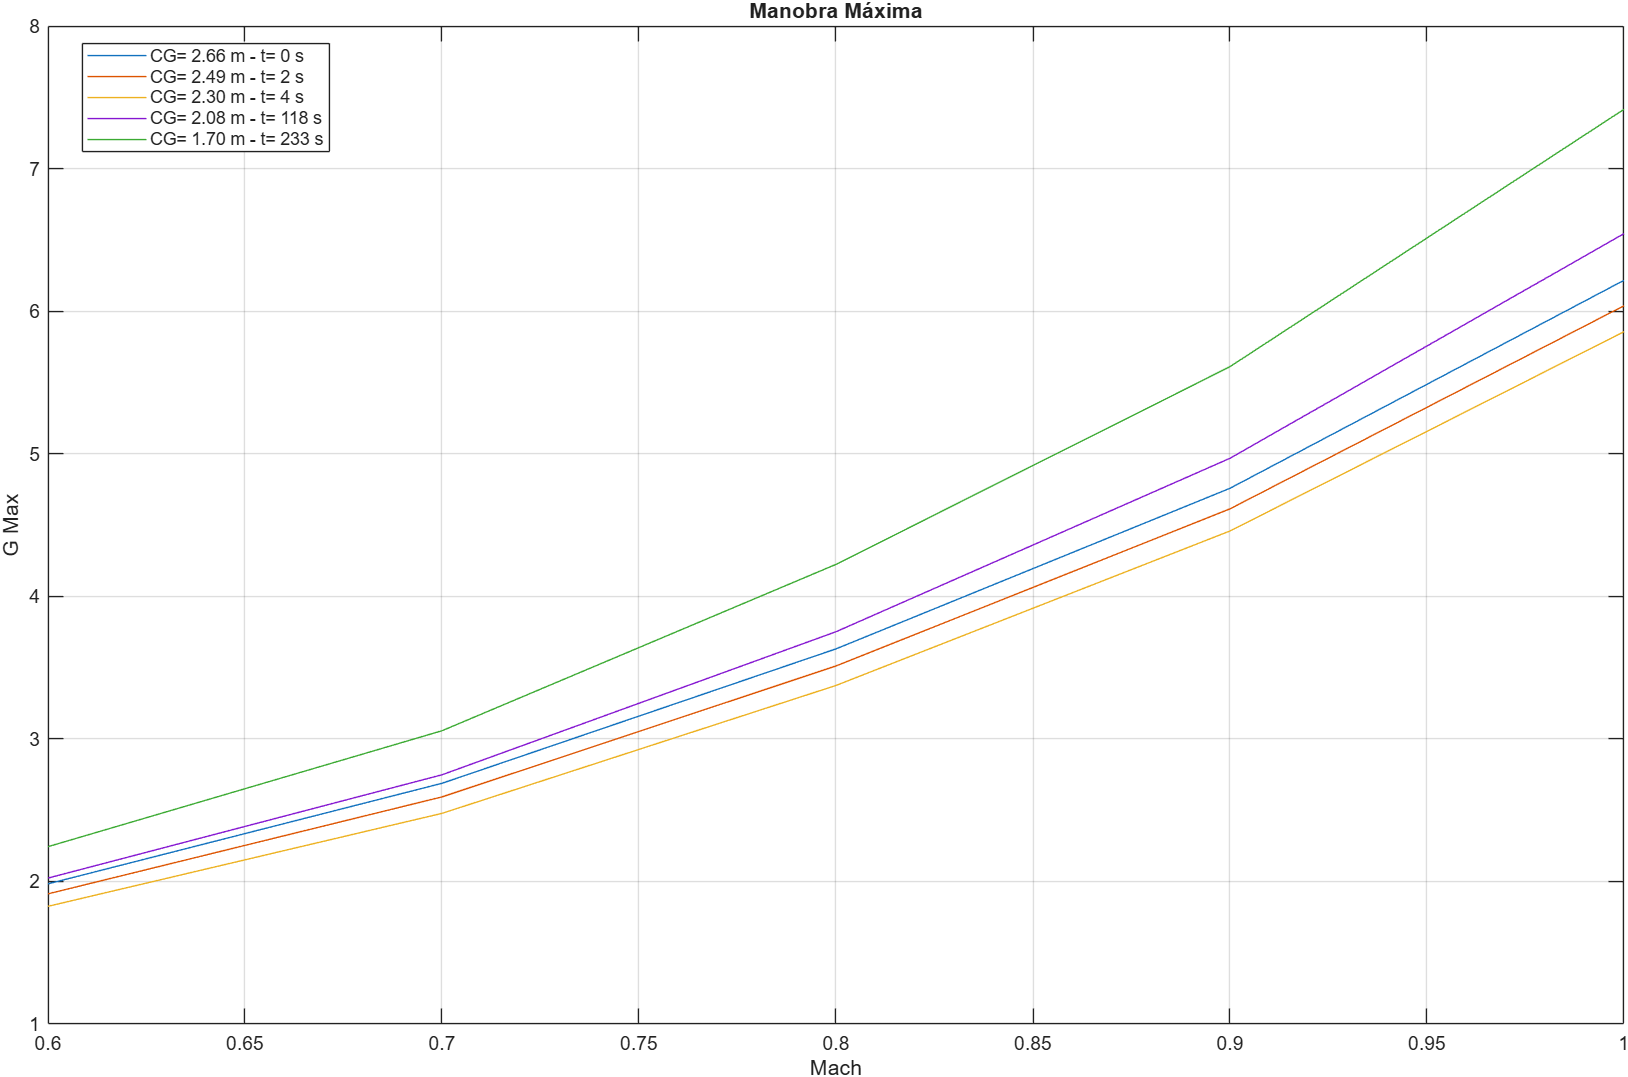
\includegraphics[width=0.82\textwidth]{figures/gmax.png}
\caption{Maximum maneuver $G_{max}$ versus Mach for the five CG phases. All curves trim within $\pm 20^\circ$.}
\end{figure}
